\documentclass[a4paper,
  twoside, % two have to sided mode (odd and even page numbers)
  headlines=2.1 % number of lines in the heading, increase if you want more
  ]{scrartcl}

% Packages
\usepackage[english]{babel}
\usepackage[utf8]{inputenc}
\usepackage[T1]{fontenc}
\usepackage{siunitx}
\usepackage{lipsum}
\usepackage[left=2.5cm,right=2.5cm,top=2.5cm,bottom=2.5cm]{geometry}
\usepackage[onehalfspacing]{setspace}
\usepackage{lmodern}
\usepackage[automark,headsepline]{scrlayer-scrpage}
\usepackage[numbers]{natbib}
\usepackage{csquotes}
\usepackage{textcomp}
\usepackage{hyperref}
\usepackage{graphicx}
\usepackage{cleveref}
\usepackage{float}

% Commands
%\setlength{\parskip}{1em}
\setlength\parindent{0pt}

\newcommand{\yourname}{Marc Johannes Aslan \and Thomas Kötzner}
\newcommand{\headingname}{Marc Johannes Aslan, Thomas Kötzner}
\newcommand{\lecture}{MST Technologies and Processes, Assignments, course winter semester 2018/2019}
\author{\yourname}
\title{\lecture}

\pagestyle{scrheadings}
\setkomafont{pagehead}{\normalfont}
\lohead{\lecture\\\today}
\lehead{\lecture\\\today}
\rohead{\\}
\rehead{\\}

\title{MST Technolgies and Processes}
\subtitle{Assignment \#2: High aspect ratio MEMS}
\date{\today}
\author{Thomas Kötzner, Marc Johannes Aslan}
\date{January 2019}

\begin{document}

\maketitle

\section{Task}
The aim of this assignement is to introduce and describe high aspect ratio MEMS. Furthermore, typlical applications of high aspect ratio MEMS are presented. Finally, methods are shown with which high aspect ratio MEMS structures can be produced. This involves methods for different materials such as metals, polymers and semiconductors.

\section{Introduction}
As Richard Feynman already stated in his famous lecture \enquote{There's plenty of room at the bottom} in 1960, that there should be a field, in which it is possible to manipulate matter on an atomic scale. \cite{feynman2012} With these techniques, it should be possible to build nanoscale machines or sensors. Nearly 60 years later, this field is known as micro systems technology, where such tiny structures are typical and used for different applications. To achieve manufacturing such devices, there are plenty different technologies. For each of them, there are certain advantages and disadvantages, which are also dependent of the different applications. In most cases it is typical to use high aspect ratio micro structure technology (HARMST). HARMST devices are required for a number of common applications like sensors. The improvement in plasma techniques made the fabrication of such structures possible. 

\section{High aspect ratio micro structure technolgy}
Aspect ratio is described as ratio between the depth or rather height and the minimal lateral expansion of the structure. In some publications high aspect ratio is defined bigger than 10:1. \cite{mcnie2000} One advantage of high aspect ratio is the increased flexibility in 3 dimensions. It is possible to build structures of different shapes and varying heights or widths. This is often used for applications with high packaging density, using the height rather the width reduces the needed space on the substrate.\cite{mcnie2000} Due to the increased height, which offers bigger areas, it is possible to increase the capacitance of the structures, which is needed in many applications. Bigger capacities are required for applications with lower driving voltages. Also, the sensitivity is improved, e.g. in applications where micro mechanical motions should be detected, because it is easier to detect changes in bigger capacities. \cite{pang2001} For applications in critical areas like medical technology or automotive, high aspect ratio provides high security. It prevents e.g. cross axis coupling or immunity to high frequency and high amplitude parasitic effects. \cite{mcnie2000,NXP2009}. Furthermore, high aspect ratio provides an exceptional signal-to-noise ratio and over-damped mechanical response. \cite{NXP2009} Another characteristic of high aspect ratio is the possibility to build thick high mass elements. Those are often used to increase mechanical stability, which leads to more robustness. Also, released features of MEMS can be formed, where the stress due to bending is reduced. \cite{mcnie2000, pang2001, hutchison2010} Typical production processes for these structures are \enquote{Deep Reactive Ion Etching} (DRIE), \enquote{Lithographie, Galvanik und Abformung} (LIGA) and \enquote{Single Crystal Reactive Etching And Metallization} (SCREAM). According to the process, higher ratios could be reached and several materials are editable. Nevertheless, it must be said, that those processes are more complex and expensive than techniques like conventional dry etching or lithography. On top of that, the planning effort to design these structures is bigger, because it is necessary to take care of effects like the critical aspect ratio. Important parameters are e.g. are the own weight of the structures, inertia, angles of released features to the substrate and shear effects.

\section{Applications}
There are plenty of applications for microstructures with a high aspect ratio. These are using therefore specific advantages of high aspect ratio. Micro inertial sensors is one big area of applications using high aspect ratio structures. The group of micro inertial sensors includes, among others, accelerometers, gyroscopes, angular rate sensors etc. Especially in the automotive industry, these sensors are often used and have therefore been developed steadily over the years.
\begin{figure}[H]
    \centering
    \begin{minipage}{.5\textwidth}
        \centering
        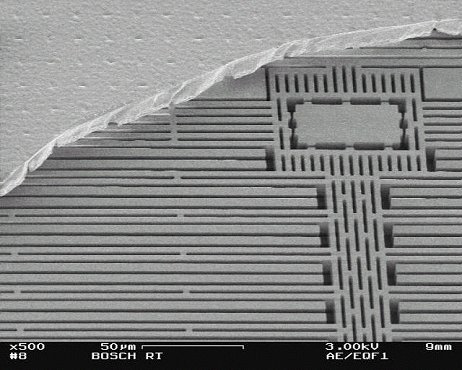
\includegraphics[height = 175px]{Graphics/Accelerometer.png}
        \caption{Accelerometer \cite{sensors2018}}
        \label{fig:accelerometer}
    \end{minipage}%
    \begin{minipage}{0.5\textwidth}
        \centering
        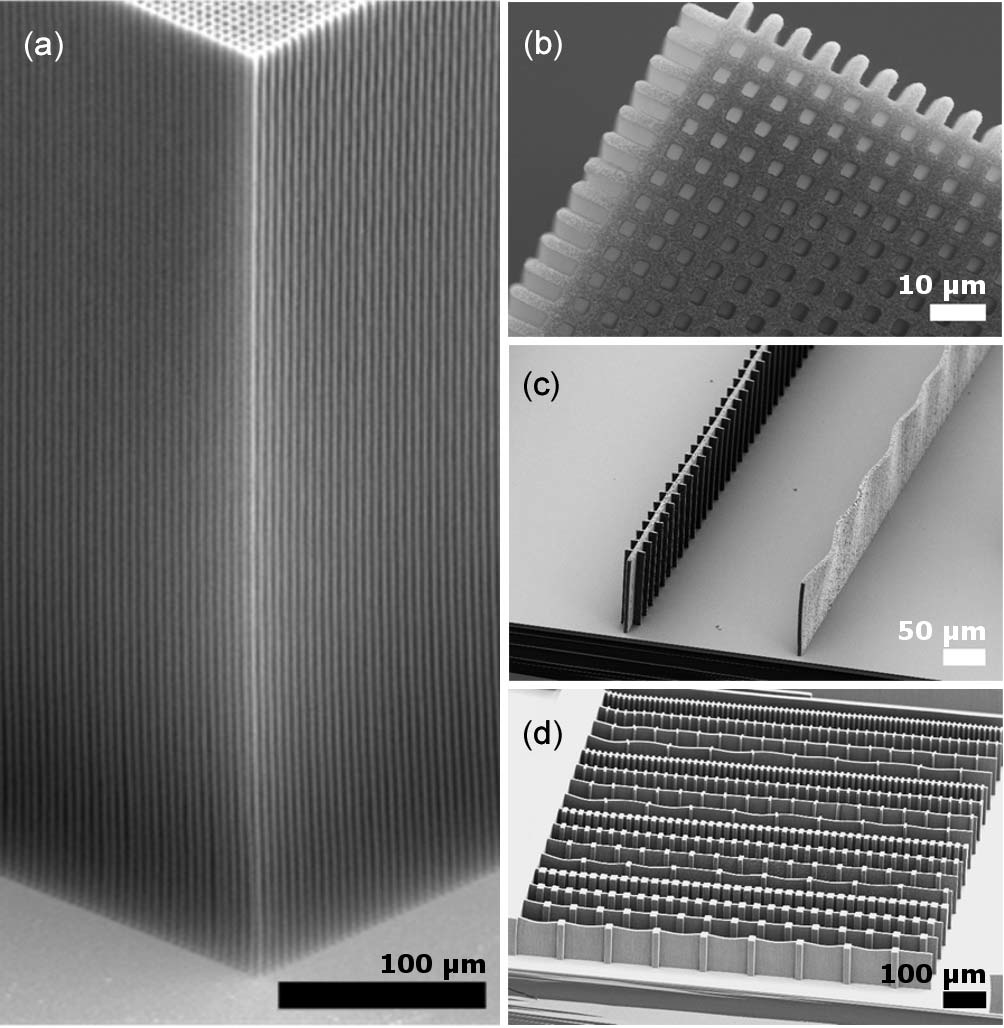
\includegraphics[height = 175px]{Graphics/nanotubes.png}
        \caption{Nanotubes \cite{hutchison2010}}
        \label{fig:nanotubes}
    \end{minipage}
\end{figure}
As seen in figure \ref{fig:accelerometer}, in acceleromters high aspect ratio structures are used for the comb structure, consiting of a movable beam in the center and attached fingers, and an anchored finger structure. Together, these structures form capacities. If the beam moves, it is possible to measure decreasing and increasing capacities. With high aspect ratio structures, sensing of these changes is getting easier, and the performance of inertial sensors can be increased massively.

Another application is e.g. Nanotubes, as seen in figure \ref{fig:nanotubes}. These can be used as a framework for fabrication of other microstructures with a high aspect ratio. \cite{hutchison2010}

Further applications are 3D-circuit integration, where it is possible to realize circuit paths with a high aspect ratio \cite{wikiDRIE}, released microstructure features etc.

\section{Fabrication methods}

\subsection{Metals}
\subsubsection{LIGA}
A very old fabrication process for producing structures with a high aspect ratio is synchrotron radiation lithography, galvanoforming, and plastic moulding, also known as LIGA process. It was developed by researchers from Karlsruhe and presented to the scientific community as early as 1986. \cite{BECKER198635} Originally developed as a process for uranium enrichment, it has quickly become a widely used process for producing high aspect ratio microstructures. It is possible to differentiate between two different variants of LIGA: The first variant is based on X-rays produced by a synchrotron, as in the original method. The second method is an enhancement of X-ray LIGA and is based on UV radiation. This procedure is discussed in section \ref{uv_liga}. X-ray LIGA enables over 100:1 aspect ratios and applies to metals, polymers and semiconductor substrates. The process is now extremely complex and has been continuously developed, a rough overview of the different production steps is given below.
\begin{figure}[H]
	\centering
	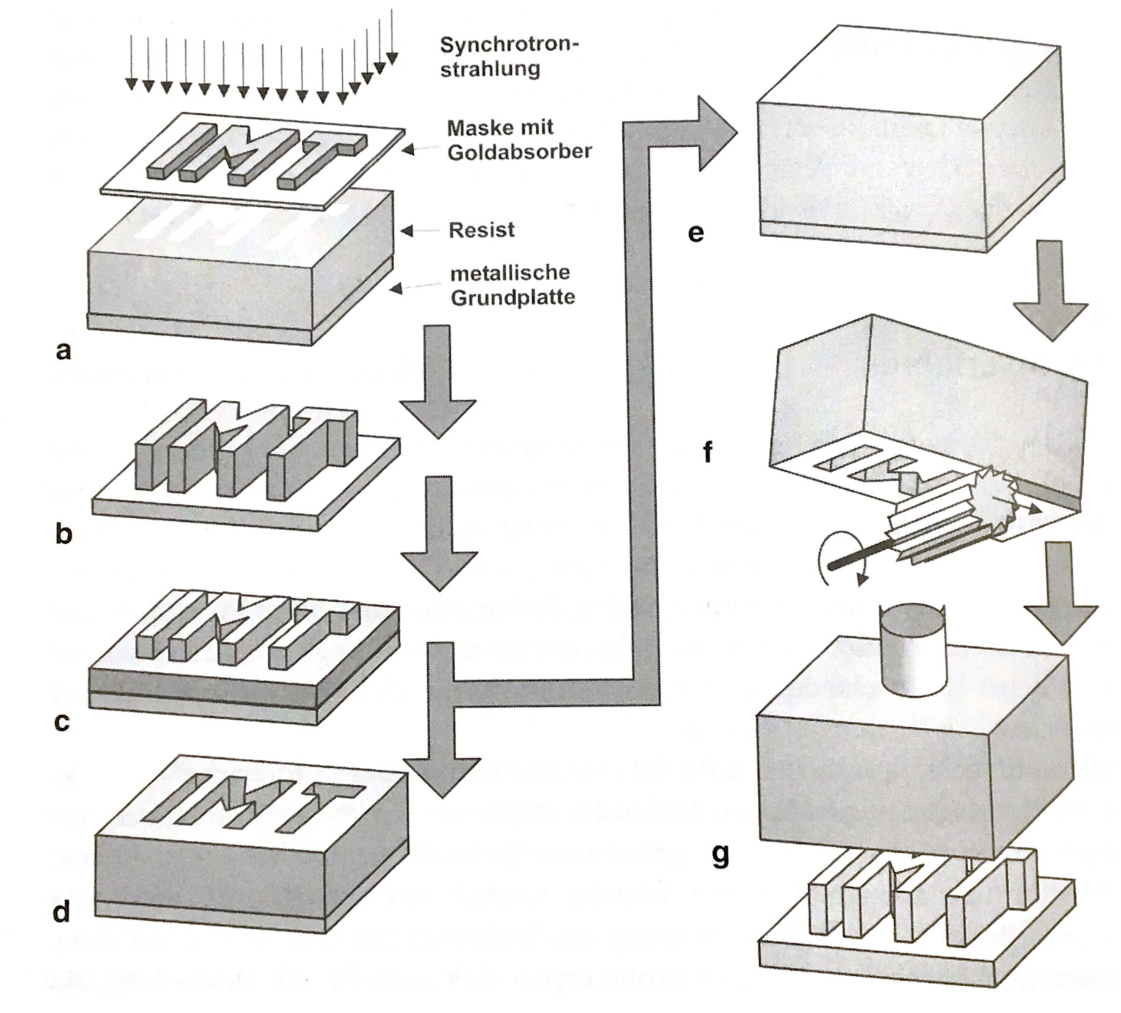
\includegraphics[width=0.5\textwidth]{Graphics/Liga/LIGA.pdf}
	\caption{Process steps LIGA\cite{menz2005paul}}
	\centering
	\label{Schematic_LIGA}
\end{figure} 
The first process step of LIGA, as it is in the name, is lithography. In the case of X-ray LIGA, one therefore also uses X-ray lithography. Starting on a flat substrate, the first process step is to apply a conductive layer on the substrate. This layer is called seed-layer. For this step, typical processes are sputtering and evaporation. If necessary, an adhesive layer can also be applied to the substrate before that. After this step, a photoresitive material is applied to the substrate. The photoresist has to meet many requirements, in most cases PMMA is used. The next process step after the application of the photoresist coating is the exposure with X-rays, generated by the synchrotron source. This is also a very complex process step, depending on many effects like diffraction or substrate fluorescence. This is the reason why the mask for exposure also has to meet many requirements. After this step, the photoresist is exposed by a certain pattern determined by the mask and can be developed. The lithography step ends by developing the resist and is followed by the electroplating step. Here, the negative form, which remains due to the removed photoresist, is filled upwards with metal by electroplating. It is possible to use different metals like gold, nickel, copper etc. After stripping of the remaining photoresist, which is a lengthy chemical process, it is possible to continue with etching the seed-layer, or using further electroplating. This depends on the application. \cite{BECKER198635, menz2005paul}

As seen here, LIGA is a very complex fabrication process. One big advantage is the possibility to produce microstructures with a high aspect ratio, also with different thicknesses. Disadvantages are the high complexity, the expensive equipement and the slow process speed.

\subsection{Polymers}
As with metals, LIGA can also be used in polymers. Another option is the usage of Hot embossing, as a method specialized for the fabrication of polymer high aspect ratio structures. This technique is based on stamping a certain pattern into a polymer. For this, the fabrication of an embossing master is necessary, which can be produced by common techniques like LIGA or DRIE. The embossing master acts as a negative form and is mounted to the embossing tool. After heating up the polymer , the tool is brought into contact with the polymer and then embossed with a certain force. After cooling down the polymer, the tool is taken out, and the high aspect ratio structure remains in the polymer. \cite{BECKER2000130}

The usage of polymer high aspect ratio structures brings the ability to take all advantages of polymers microstructures, which are often uses e.g. in medicine. The method of hot embossing is a very cheap alternative to common processes like LIGA and DRIE.

\subsection{Semiconductor materials}
\subsubsection{Deep Reactive Ion Etching (DRIE)}\label{DRIE}
Deep Reative Ion Etching is an enhancement of reactive Ion Etching and was developed by Robert Bosch AG in 1990. This anisotropic process is the most common technique to produce an very high aspect ratio on silicon. An aspect ratio up to 50:1 is achievable. This aspect ratio is not as high like in the LIGA process, but the advantages of DIRE are cost savings and faster process time. Also the previously mentioned aspect ratio is high enough for the most applications, like  Microsystems and 3D-Integration of electrical circuits. It is possible to etch 20 \textmu m per minute, but usually the substrate is etched with a speed of 1-2 \textmu m per minute, to get more precision and less wave-like structures on the side walls of the etching channel\cite{wikiDRIE}. An simplified process discretion is shown in Figure \ref{Schematic_drie}. First of all, what is not mentioned in the figure, a mask is attached to the substrate, which protects the areas which should not be etched. After that, the first etching step is performed with SF\textsubscript{6}. The echting gas is removed and CF\textsubscript{4} is lead to the substrates. The gas reacts in an isotropic process with the silicon and builds a protecting plasma-polymer-layer on the top of the whole substrate as seen in Figure \ref{Schematic_drie} Phase 1. To etch the next step, the previously mentioned anisotropic etching process will be repeated. Because of the anisotropic characteristic the SF\textsubscript{6} is etching through the protection layer at the bottom into the substrate, while the walls are nearly untouched. The three phases are repeated until the desired depth is reached. A disadvantage of this process is the litigation. It has to be optimized for every single structure, to get vertical and smooth side walls\cite{menz2005paul}.

\begin{figure}[H]
	\centering
	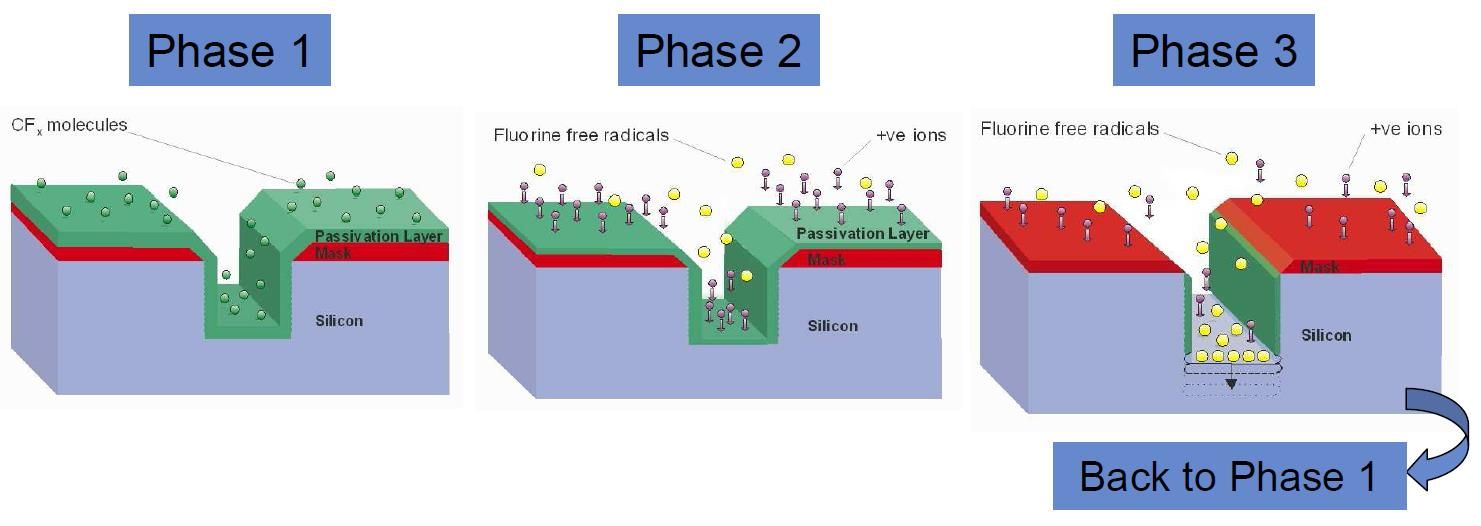
\includegraphics[width=\textwidth]{Graphics/DIRE/drie-schema_fraunhofer.jpg}
	\caption{Schematic representation of DRIE \cite{Fraunhofer2019}}
	\centering
	\label{Schematic_drie}
\end{figure} 

\subsubsection{UV LIGA}\label{uv_liga}
UV-LIGA is an enhancement of X-Ray LIGA to create microstructures on semiconductors. The general variance to X-Ray-LIGA is the use of epoxy-based SU-8 photoresist. Using this photoresist has enabled the fabrication of tall and high aspect ratio structures without the use of a very expensive synchrotron source\cite{genolet2014uv}. UV LIGA is not as precisely as X-Ray LIGA and less aspect ratio is achievable, but according to the processing costs, this limitations are acceptable\cite{wikiUVLiga}.

\subsubsection{SCREAM}
Another process to get high aspect ratios on semiconductors is SCREAM (Single Crystal silicon Reactive Etching an Metallization). It is used for under etched structures like beams and bridges. After DRIE (Section\ref{DRIE}) a silicon oxide layer is exposed, to protect the side walls and the bottom. The following anisotropic etching step removes the silicon oxide at the bottom, while the subsequent isotropic etching step undermines the material between the trenches. The top layer is untouched and the floating structure is suspended at the ends because of the mask\cite{menz2005paul}. With SCREAM an aspect ratio >50:1 can be reached, very large, robust and stiff vertical movable structures can be created and dry etching methods are used, which brings more flexibility(reference). Disadvantages are low quality factor because of high damping of the silicon dioxide layers and thermal stress can occur because of different materials which are used\cite{macdonald1996scream}.

\section{Conclusion}
This paper discussed high aspect ratio MEMS. A lot of positive arguments, like increased flexibility in 3 dimensions and possibility to increase the capacitance of the structures without needing more surface area, what results in higher sensitivity, but also negative points like high production costs and times are mentioned. The assignment contains applications of HARMST and describes fabrication processes belonging to the materials on which they are applied. In conclusion, it can be said that the use of high aspect ration must be weighed up in advance on the basis of the application in order to avoid unnecessary costs.


\bibliography{literature}
\bibliographystyle{IEEEtran}


\end{document}
